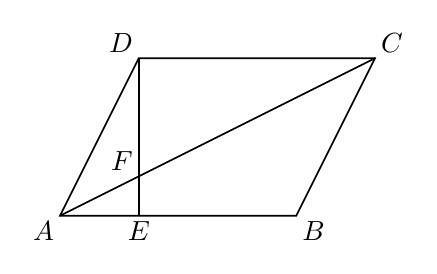
\begin{tikzpicture}[x=1cm,y=1cm,font=\normalsize,
 geometry edge/.style={solid,line width=.6pt},
 geometry mark/.style={solid,line width=.6pt},
 geometry label/.style={font=\normalsize,inner sep=2pt}]
\coordinate (A) at (0.0000,0.0000);
\coordinate (B) at (3.0000,0.0000);
\coordinate (D) at (1.0000,2.0000);
\coordinate (C) at (4.0000,2.0000);
\coordinate (E) at (1.0000,0.0000);
\coordinate (F) at (1.0000,0.5000);
\draw[geometry edge] (A)--(B)--(C)--(D)--cycle;
\draw[geometry edge] (D)--(E);
\draw[geometry edge] (A)--(C);
\node[geometry label,below left] at (A) {$A$};
\node[geometry label,below right] at (B) {$B$};
\node[geometry label,above right] at (C) {$C$};
\node[geometry label,above left] at (D) {$D$};
\node[geometry label,below] at (E) {$E$};
\node[geometry label,above left] at (F) {$F$};
\end{tikzpicture}
